\PassOptionsToPackage{hidelinks}{hyperref}

\documentclass[stu,12pt,floatsintext]{apa7} % man doc stu jou

\usepackage[american]{babel}

\usepackage{csquotes} 
\usepackage[style=apa,sortcites=true,sorting=nyt,backend=biber]{biblatex}

\DeclareLanguageMapping{american}{american-apa}
% \addbibresource{bibliography.bib} 
\usepackage[T1]{fontenc} 
\usepackage{ctex}
\usepackage{xeCJK}
\usepackage{mathptmx} % This is the Times New Roman font, which was the norm back in my day. If you'd like to use a different font, the options are laid out here: https://www.overleaf.com/learn/latex/Font_typefaces
% Alternately, you can comment out or delete these two commands and just use the Overleaf default font. So many choices!
\setCJKmainfont{Songti SC Regular} % 设置中文主字体为 STSong,字间距增加
\setmainfont{Times New Roman} % 设置英文字体
% \renewcommand{\today}{\number\year 年 \number\month 月 \number\day 日}


\usepackage{enumitem}
\usepackage{amsmath}
\usepackage{amssymb}


% Set up fancy header/footer
\usepackage{fancyhdr}
\pagestyle{fancy}
\fancyhead[LO,L]{2025年春学期}
\fancyhead[CO,C]{贝叶斯统计学基础}
\fancyhead[RO,R]{\today}
\fancyfoot[LO,L]{}
\fancyfoot[CO,C]{\thepage}
\fancyfoot[RO,R]{}
\renewcommand{\headrulewidth}{0.4pt}
\renewcommand{\footrulewidth}{0.4pt}
% 设置首行缩进为一个字符宽度
\setlength{\parindent}{1em} % 1em 约等于一个字符宽度


% Title page stuff _____________________
\title{APA Format Starter Paper, Tailored to Lab Reports But Adaptable to Other Writing Assignments} % The big, long version of the title for the title page
\shorttitle{APA Starter} % The short title for the header
\author{Your Name Here}
\duedate{April 20, 2024}
% \date{January 17, 2024} The student version doesn't use the \date command, for whatever reason
\affiliation{Your School}
\course{PSY 4321} % LaTeX gets annoyed (i.e., throws a grumble-error) if this is blank, so I put something here. However, if your instructor will mark you off for this being on the title page, you can leave this entry blank (delete the PSY 4321, but leave the command), and just make peace with the error that will happen. It won't break the document.
\professor{Dr. Professor}  % Same situation as for the course info. Some instructors want this, some absolutely don't and will take off points. So do what you gotta.

\abstract{This is the abstract for this paper, wherein the main points of the introduction, method, results, and discussion are quickly talked about. Probably in more than one sentence, though. Dare I guess, more than two? There is a page break before starting the Introduction.}

%\keywords{APA style, demonstration} % If you need to have keywords for your paper, delete the % at the start of this line


\begin{document}
\begin{titlepage}
    \centering
    \vspace*{4cm} % 调整标题的垂直位置
    \Huge
    {\heiti 贝叶斯统计学基础作业2} \\
    \vspace{1cm}
    \Large
    毛沛炫\ \ \ 3220102692 \\
    \vspace{12.3cm}
    \Large
    % \today
    \number\year 年 \number\month 月 \number\day 日
    \vfill
\end{titlepage}

\xeCJKsetup{CJKglue={\hskip 0.8pt plus 0.08\baselineskip}}

\noindent 1. {\heiti 假定对于二项分布参数\textit{p}我们采用均匀先验分布,并且在 10次试验中观察到了 4 次正性结果,}
\begin{enumerate}[itemsep=2pt,topsep=0pt,parsep=0pt,label=(\alph*)]
\item  给出先验贝塔分布的参数值(2 分)

\item  给出后验贝塔分布的参数值(2 分)
    
\item  给出在先验分布下二项分布参数 \textit{p} 的期望值(2 分)
    
\item  给出样本中正性结果的比例(2 分)
    
\item  给出二项分布参数 \textit{p} 的极大似然估计值(2 分)
    
\item  给出在后验分布下二项参数 \textit{p} 的期望值,并以先验分布下该参数的期望值和该参数的极大似然估计值的加权平均形式表达(4 分)
\end{enumerate}


\textbf{解答:}
\begin{enumerate}[itemsep=2pt,topsep=0pt,parsep=0pt,label=(\alph*)]
    \item 先验贝塔分布的参数值
    
    \begin{figure}
        \centering
        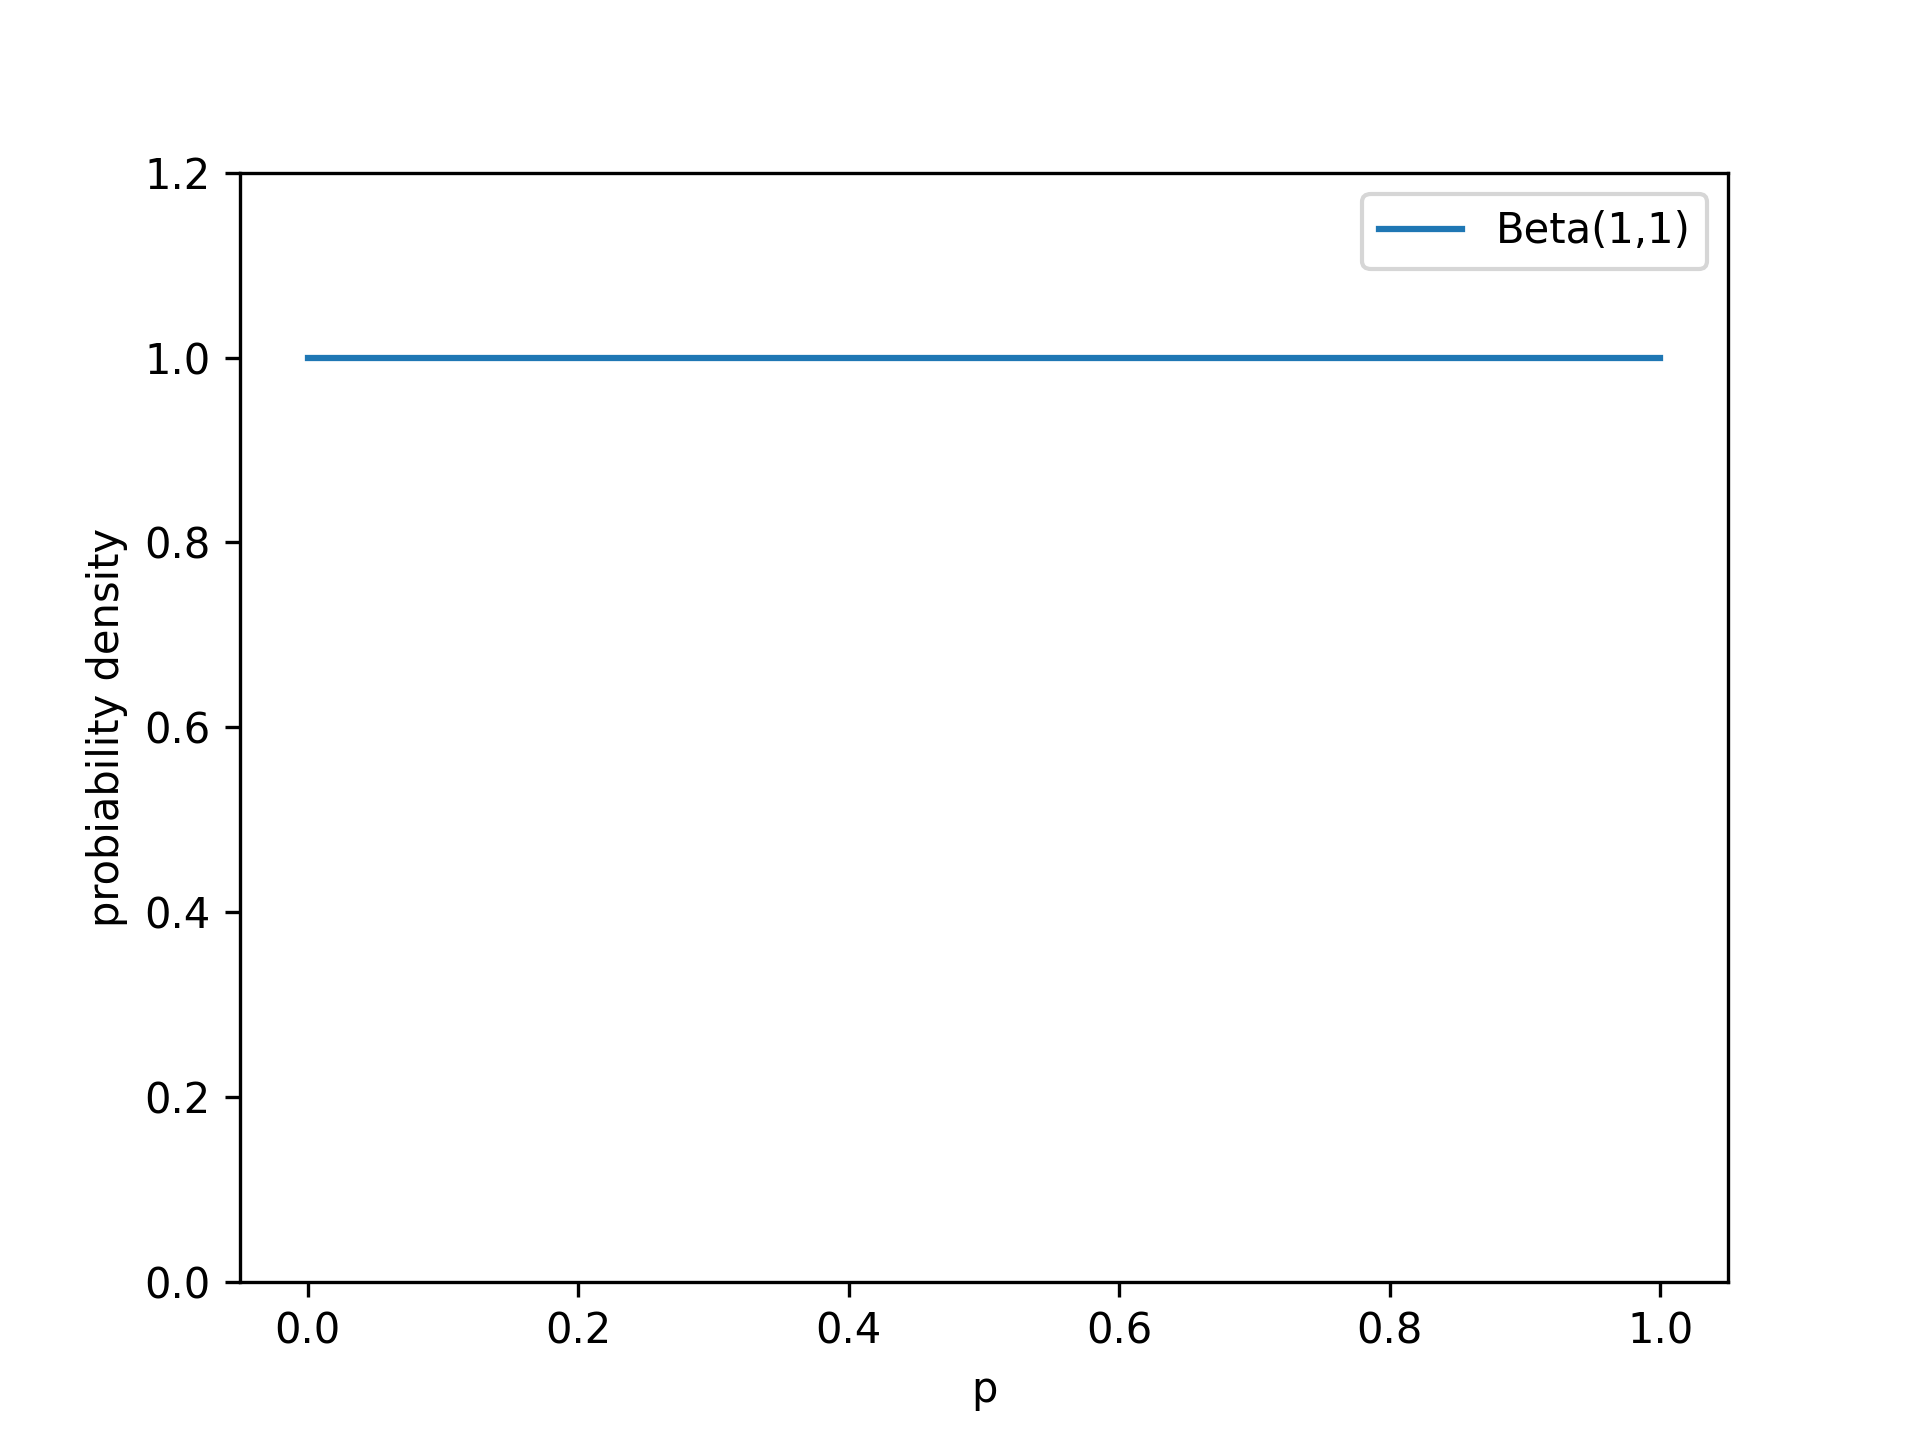
\includegraphics[width=0.6\linewidth]{figure/beta11.png} % Replace with the actual path to your image
        \caption{先验贝塔分布的参数值} % Replace with your caption
        \label{fig:beta11} % Ensure the label is inside the figure environment
    \end{figure}
    \(\alpha = 1\) 和 \(\beta = 1\)。见图\ref{fig:beta11}

    \item 后验贝塔分布的参数值
    
    \begin{figure}
        \centering
        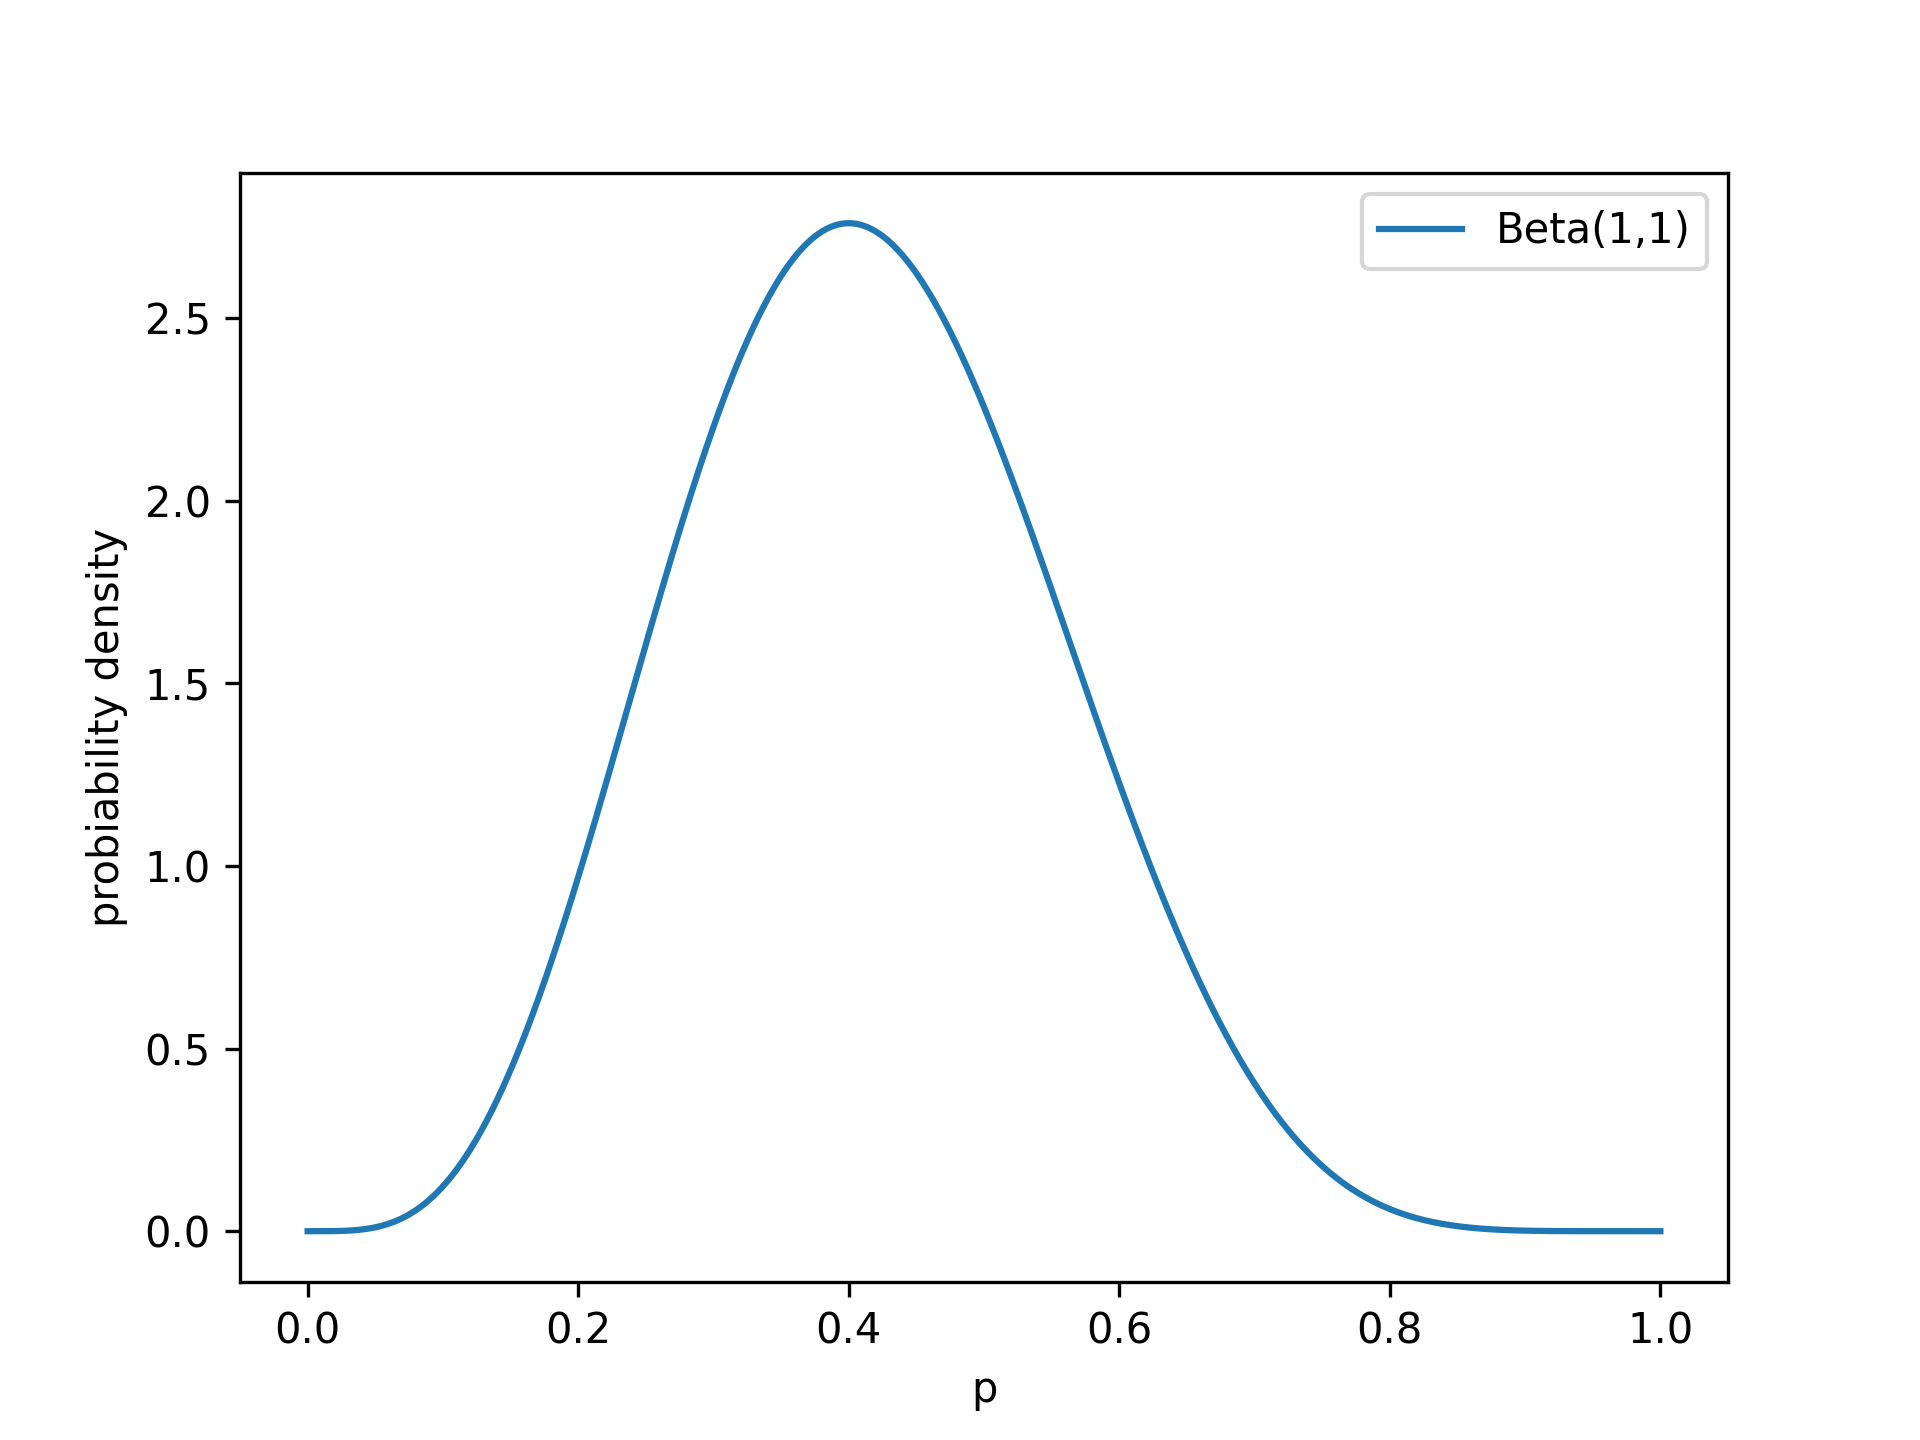
\includegraphics[width=0.6\linewidth]{figure/beta57.png} 
        \caption{后验贝塔分布的参数值}
        \label{fig:beta57}
    \end{figure}
    后验贝塔分布的参数为 \(\alpha = 5\) 和 \(\beta = 7\)。
    \[
    \alpha_{\text{后验}} = \alpha + \text{正性结果数} = 1 + 4 = 5
    \]
    \[
    \beta_{\text{后验}} = \beta + \text{负性结果数} = 1 + 6 = 7
    \]


    \item 给出二项分布参数 \textit{p} 的期望值
    
    \begin{align}
        f(x) & = p^x(1-p)^{1-x} \\
        L(x_1, x_2, \cdots, x_n; ) & = \prod_{i=1}^{n} p^{x_i}(1-p)^{1-x_i} \\
    \end{align}

    \item 给出样本中正性结果的比例
    
    \item  给出二项分布参数 \textit{p} 的极大似然估计值
    
    \item  给出在后验分布下二项参数 \textit{p} 的期望值,并以先验分布下该参数的期望值和该参数的极大似然估计值的加权平均形式表达

\end{enumerate}


1. \textbf{先验贝塔分布的参数值}

对于均匀先验分布,贝塔分布的参数为 \(\alpha = 1\) 和 \(\beta = 1\)。

\[
\alpha = 1, \quad \beta = 1
\]

2. \textbf{后验贝塔分布的参数值}

在观察到 4 次正性结果和 6 次负性结果后,后验贝塔分布的参数更新为:

\[
\alpha_{\text{后验}} = \alpha + \text{正性结果数} = 1 + 4 = 5
\]
\[
\beta_{\text{后验}} = \beta + \text{负性结果数} = 1 + 6 = 7
\]

因此,后验贝塔分布的参数为 \(\alpha = 5\) 和 \(\beta = 7\)。

3. \textbf{先验分布下二项分布参数 \(p\) 的期望值}

先验分布为均匀分布,其期望值为:

\[
E[p] = \frac{\alpha}{\alpha + \beta} = \frac{1}{1 + 1} = 0.5
\]

4. \textbf{样本中正性结果的比例}

样本中正性结果的比例为:

\[
\frac{\text{正性结果数}}{\text{总试验数}} = \frac{4}{10} = 0.4
\]

5. \textbf{二项分布参数 \(p\) 的极大似然估计值}

极大似然估计值为样本中正性结果的比例:

\[
\hat{p}_{\text{MLE}} = \frac{4}{10} = 0.4
\]

6. \textbf{后验分布下二项参数 \(p\) 的期望值}

后验分布的期望值为:

\[
E[p \mid \text{数据}] = \frac{\alpha_{\text{后验}}}{\alpha_{\text{后验}} + \beta_{\text{后验}}} = \frac{5}{5 + 7} = \frac{5}{12} \approx 0.4167
\]

这个期望值可以表示为先验期望值和极大似然估计值的加权平均:

\[
E[p \mid \text{数据}] = \frac{\alpha + \text{正性结果数}}{\alpha + \beta + \text{总试验数}} = \frac{1 + 4}{1 + 1 + 10} = \frac{5}{12}
\]

也可以表示为:

\[
E[p \mid \text{数据}] = \frac{\text{先验权重} \times \text{先验期望} + \text{数据权重} \times \text{极大似然估计}}{\text{先验权重} + \text{数据权重}}
\]

其中,先验权重为 \(\alpha + \beta = 2\),数据权重为试验次数 \(n = 10\)。

\[
E[p \mid \text{数据}] = \frac{2 \times 0.5 + 10 \times 0.4}{2 + 10} = \frac{1 + 4}{12} = \frac{5}{12} \approx 0.4167
\]

\end{document}
